\documentclass[12pt]{article}
\usepackage{amsmath}
\newcommand{\myvec}[1]{\ensuremath{\begin{pmatrix}#1\end{pmatrix}}}
\newcommand{\mydet}[1]{\ensuremath{\begin{vmatrix}#1\end{vmatrix}}}
\newcommand{\solution}{\noindent \textbf{Solution: }}
\providecommand{\brak}[1]{\ensuremath{\left(#1\right)}}
\providecommand{\norm}[1]{\left\lVert#1\right\rVert}
\let\vec\mathbf
\usepackage{graphicx}
\usepackage{float}

\title{Linear equation in two variables}
\author{potnuru deekshitha (potnurudeekshitha@sriprakashschools.com)}

\begin{document}
\maketitle
\section*{10$^{th}$ Maths - Chapter 7}
This is Problem-2 from Exercise 7.2
\begin{enumerate}
\item  Find the coordinates of the point of trisection joining (4,-1),(-2,-3)

\solution\\
Case-1\\
$\vec{A}$=\myvec{4\\-1}, $\vec{B}$=\myvec{-2\\-3},
$m_1:m_2=2:1$
\begin{align}
&P=\frac{m_1\vec{B}+m_2\vec{A}}{m_1+m_2}\\
&P=\frac{2\myvec{-2\\-3}+1\myvec{4\\-1}}{2+1}\\
&P=\frac{\myvec{-4\\-6}+\myvec{4\\-1}}{3}\\
&P=\frac{\myvec{0\\-7}}{3}\\
&P=\myvec{0\\\frac{-7}{3}}\\
\end{align}

Case-2\\
$\vec{A}$=\myvec{4\\-1}, $\vec{B}$=\myvec{-2\\-3},
$m_1:m_2=1:2$
\begin{align}
&P=\frac{m_1\vec{B}+m_2\vec{A}}{m_1+m_2}\\
&P=\frac{1\myvec{-2\\-3}+2\myvec{4\\-1}}{2+1}\\
&P=\frac{\myvec{-2\\-3}+\myvec{8\\-2}}{3}\\
&P=\frac{\myvec{6\\-5}}{3}\\
&P=\myvec{2\\\frac{-5}{3}}\\
\end{align}



\end{enumerate}
\begin{figure}[H]
			\centering
			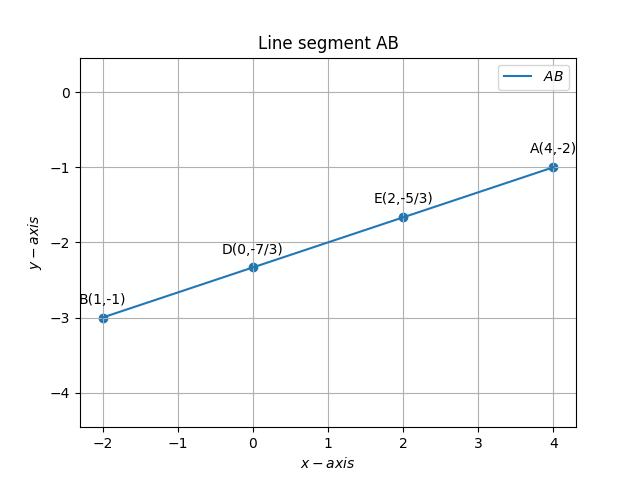
\includegraphics[width=\columnwidth]{figs/Figure_1.png}
			\caption{Line segment AB.}
			\label{fig:14}
   \end{figure}
\end{document}
